\documentclass[oneside,a4paper,titlepage]{scrartcl} % Format fuer Titelseite und Dokument (Koma-Script)
\usepackage[ngerman]{babel}                         % Sprache
\usepackage[utf8]{inputenc}                         % Direkte Eingabe von Umlauten Dokument
\usepackage[T1]{fontenc}                            % Silbentrennung auch bei Woertern mit Umlauten
\usepackage{graphicx}                               % Bilder
\usepackage{listings}                               % Aufzaehlungen
\usepackage{xcolor}                                 % Farbgebung des Sourcodes
\usepackage{lmodern}                                % Formatierung des Sourcecodes
\usepackage{longtable}                              % Fuer mehrseitige Tabellen
\usepackage{booktabs}                               % Fuer mehrseitige Tabellen
\usepackage{colortbl}                               % Fuer farbige Zeilen/Reihen in Tabellen

% Formatierung fuer Tabellen
\usepackage{tabularx}
\newcolumntype{L}[1]{>{\raggedright\arraybackslash}p{#1}} % L fuer linksbuendig mit Breitenangabe
\newcolumntype{C}[1]{>{\centering\arraybackslash}p{#1}}   % C fuer zentriert mit Breitenangabe
\newcolumntype{R}[1]{>{\raggedleft\arraybackslash}p{#1}}  % R fuer rechtsbuendig mit Breitenangabe

% Fuer den automatischen Umbruch an einem Bindestrich, wie z.B. bei "Werkstueck-Sortieranlage", statt - die Zeichen "= verwenden

% Inhaltsverzeichnis anklickbar machen
\usepackage[pdftex]{hyperref}

% Beginn des Dokuments
\begin{document}

% Titelseite aufbauen
\titlehead{\flushright}
\subject{Software Engineering II\\Wintersemester 2014/2015}
\title{Handbuch für den \textbf{\emph{PUCKMASTER 2000}}} 
\subtitle{Praktikums-Gruppe: 2.3}

% Titelseite: Autoren aufbauen
\author{
\begin{small}
  \begin{tabular}{|l|l|c|L{6cm}|}
    \hline
    \rowcolor{lightgray}\textbf{Name} & \textbf{Vorname} & \textbf{Matrikel-Nr.} & \textbf{E-Mail}\\
    \hline
    \rowcolor{white}Kirstein & Katja & 2125137 & katja.kirstein@haw-hamburg.de\\
    \hline
    Kowalka & Anne-Lena & 2081899 & anne-lena.kowalka@haw-hamburg.de\\
    \hline
    Triebe & Marian & 2124897 & marian.triebe@haw-hamburg.de\\
    \hline
    Winter & Eugen & 2081992 & eugen.winter@haw-hamburg.de\\
    \hline
  \end{tabular}
\end{small}
}

% Titelseite mit Datum und Version erstellen und Seitenzahl bei 1 beginnen
\date{\today}
\maketitle

% Inhaltsverzeichnis anlegen
\thispagestyle{empty}
\tableofcontents
\newpage
\setcounter{page}{1}


\section{Allgemeine Sicherheitshinweise}
\textbf{Die Werkstück-Sortieranlage wird aus technischen Gründen in der folgenden Dokumentation als Anlage bezeichnet.\newline}
\textbf{Technische Änderungen und Ergänzungen der Beschreibung / Anleitung sind vorbehalten.\newline
Für den Inhalt wird keine Haftung übernommen, insbesondere für Schäden durch vorhandene, nicht 
vorhandene oder fehlerhafte Angaben.\newline
Weitergabe und Ergänzung dieser Beschreibung / Betriebsanleitung sind nicht gestattet, soweit nicht ausdrücklich genehmigt.\newline}
\textbf{Der Betreiber der Anlage ist verpflichtet, eine Betriebsanweisung für das Bedienungspersonal zu erstellen, um dieses vor Gefährdung der Gesundheit oder anderen sicherheitstechnischen Gefahren zu schützen. Außerdem ist der Betreiber verpflichtet, das Bedienungspersonal über die sichere und ordnungsgemäße Bedienung und den sachgerechten Betrieb der Anlage zu unterweisen.}

\newpage

\section{Einleitung}
Vielen Dank für den Erwerb des \textbf{\emph{PUCKMASTER 2000}}!\newline\newline
Dem neuesten und innovativsten Modell aus der \textbf{\emph{PUCKMASTER}}-Produktfamilie.\newline\newline
Als globaler Marktführer für Anlagen zur Sortierung von Werkstücken sind wir stolz, Ihnen mit dem \textbf{\emph{PUCKMASTER 2000}} den nächsten technischen Meilenstein auf diesem Gebiet präsentieren zu dürfen.\newline\newline
Die wichtigsten Punkte unter den zahlreichen Neuerungen sind:\newline
\begin{itemize}
  \item Verdoppelung der Bandgeschwindigkeit
  \item Doppelte Anzahl von Werkstücken
  \item Verbesserte Genauigkeit bei der Höhenmessung
  \item Vergrößerung der Rutsche für aussortierte Werkstücke
  \item Visualisierung des Betriebs mittels einer Ampelanlage
  \item Verringerung der Leistungsaufnahme durch Stand-By des Laufbandes\newline
\end{itemize}
Diese und viele weitere Neuerungen warten darauf die Leistungsfähigkeit Ihres Betriebes im Alltag zu verbessern und helfen Ihnen dabei Ihre Produktion gewinnbringend zu steigern.\newline\newline
Die Zukunft der Werkstück-Sortierung beginnt heute - bei Ihnen!\newline\newline
Viel Spaß mit Ihrem \textbf{\emph{PUCKMASTER 2000}}!

\newpage 

\section{Sicherheit}
\subsection{Allgemeines}
Es ist darauf zu achten, dass die Anlage gemäß dieser Anleitung verwendet wird. Unsachgemäße Verwendung
kann zu unerwartetem Verhalten führen und sollte vermieden werden. Für Schäden, die aus unsachgemäßem Betrieb resultieren, haftet der Betreiber, bzw. der Benutzer der Anlage.

\subsection{Sicherheitsvorrichtungen}
Die Anlage verfügt zur Wahrung der Sicherheit der Benutzer über folgende Vorrichtungen
\subsubsection{E-Stopp-Taste}
Die gesamte Anlage kann jederzeit zum Stillstand gebracht werden, indem die E-Stopp-Taste betätigt wird.\newline
\textbf{Die laufende Software wird dadurch ebenfalls beendet!}\newline
Nach Betätigung der E-Stopp-Taste muss daher die gesamte Anlage zurückgesetzt werden, bevor sie erneut in Betrieb genommen werden kann.
\subsubsection{Ampelanlage}
Jedes der beiden Förderbänder besitzt eine eigene Ampelanlage, über die sich der aktuelle Zustand des jeweiligen Förderbandes feststellen lässt.

\newpage

\section{Bestandteile der Anlage}
Die gesamte Anlage besteht aus zwei Förderbändern mit jeweils einem eigenen GEME-Rechner und den zu sortierenden Werkstücken.

\subsection{Förderband}
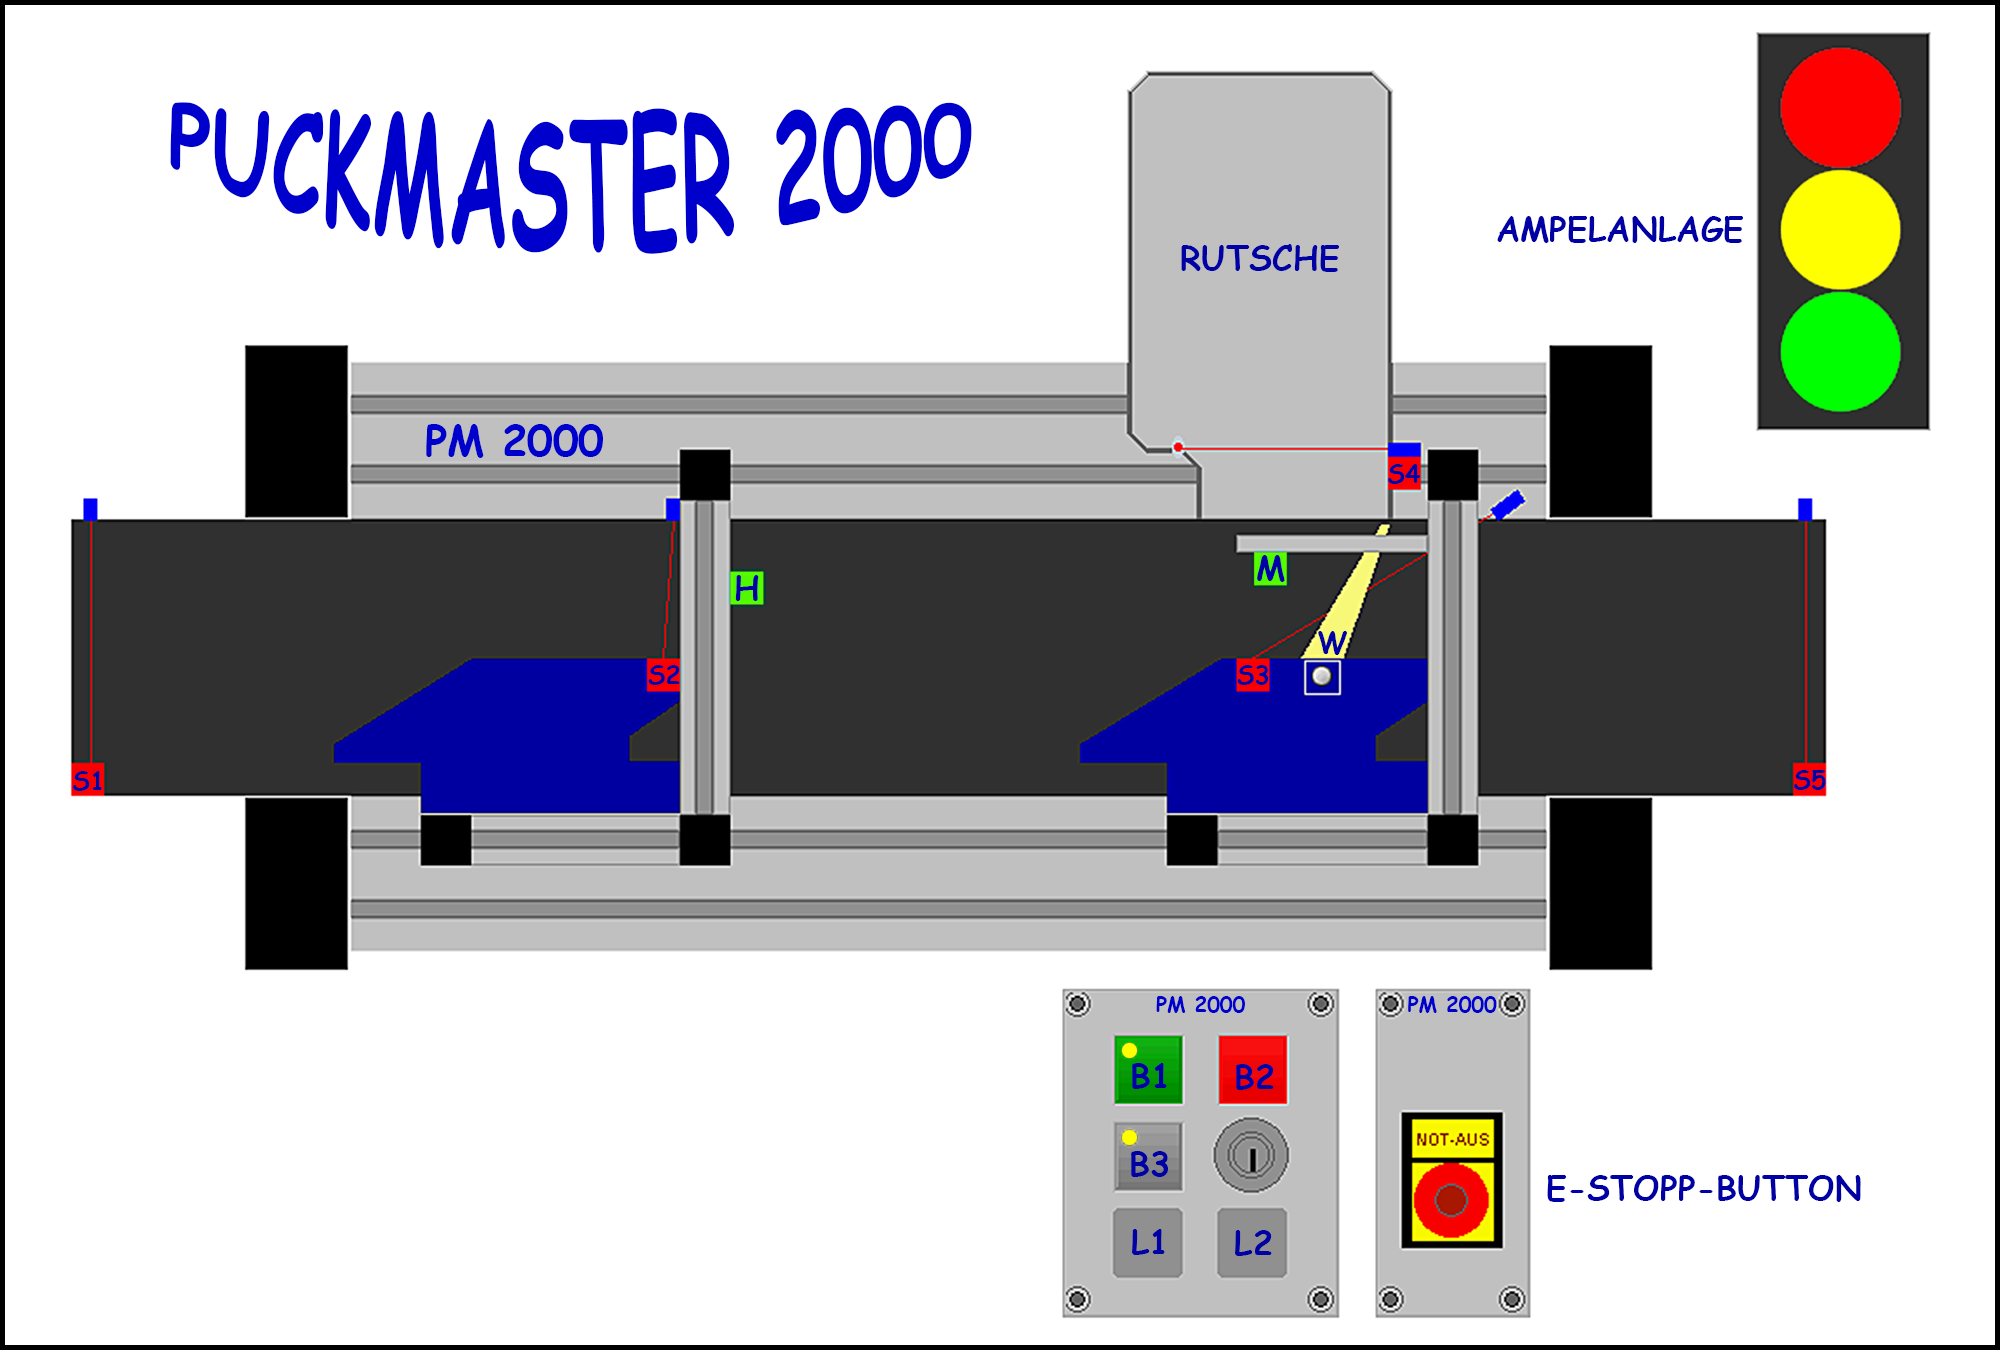
\includegraphics[scale=0.86]{imgs/PUCKMASTER_2000.png}
\newline
\newline
\begin{small}
  \begin{tabular}{|c|L{10.5cm}|}
    \hline
    \rowcolor{lightgray}\textbf{Bauteil} & \textbf{Beschreibung}\\
    \hline
    \rowcolor{white}\textbf{S1} & Lichtschranken-Sensor für den Einlauf des Förderbandes\\
    \hline
    \textbf{S2} & Lichtschranken-Sensor für den Bereich der Höhenmessung\\
    \hline
    \textbf{S3} & Lichtschranken-Sensor für den Bereich der Weiche\\
    \hline
    \textbf{S4} & Lichtschranken-Sensor für die Rutsche\\
    \hline
    \textbf{S5} & Lichtschranken-Sensor für den Auslauf des Förderbandes\\
    \hline
    \textbf{H} & Höhenmesser\\
    \hline
    \textbf{M} & Metallsensor\\
    \hline
    \textbf{W} & Weiche für das Aussortieren von ungültigen Werkstücken\\
    \hline
    \textbf{B1} & Start-Taste (mit LED)\\
    \hline
    \textbf{B2} & Stopp-Taste\\
    \hline
    \textbf{B3} & Reset-Taste (mit LED)\\
    \hline
    \textbf{L1} & LED 1\\
    \hline
    \textbf{L2} & LED 2\\
    \hline
    \textbf{E-STOPP-TASTE} & E-Stopp-Taste zum Stoppen der gesamten Anlage\\
    \hline
    \textbf{RUTSCHE} & Auffangbehältnis für ungültige Werkstücke\\
    \hline
    \textbf{AMPELANLAGE} & Anzeige für den Betriebs-Zustand des Förderbandes\\
    \hline
  \end{tabular}
\end{small}

\subsubsection{Funktionsweise des Förderbandes}
Jedes Förderband ist mit einem eigenen Motor ausgestattet. Befinden sich keine Werkstücke auf dem Förderband oder ist das Sortieren bereits abgeschlossen, schalten sich die Motoren ab um Strom zu sparen.\newline
\newline
Über die gesamte Länge eines Förderbandes sind mehrere Lichtschranken-Sensoren verteilt, um die aktuelle Position des Werkstückes bestimmen zu können.\newline
\newline
Des Weiteren verfügt jedes Förderband über einen Höhenmesser, um die Höhe eines Werkstückes bestimmen zu können.\newline
\newline
Ebenso hat jedes Förderband einen Metallsensor, mit dem erkannt werden kann, ob ein Werkstück einen Metalleinsatz besitzt.\newline
\newline
Außerdem gibt es eine Weiche, mit deren Hilfe ungültige Werkstücke über eine Rutsche aussortiert werden können.\newline
\newline
Die Kommunikation zwischen den Förderbändern erfolgt über die seriellen Schnittstellen der beiden zugehörigen GEME-Rechner, die miteinander verbunden werden.\newline
\newline
Durch die Kommunikation und die Software wird die Reihenfolge der Förderbänder und damit die Art der Sortierung festgelegt.

\subsection{Werkstücke}
Es gibt folgende Typen von Werkstücken:
\begin{itemize}
    \item Zu flache Werkstücke (ungültig, werden mit Hilfe der Weiche aussortiert)
    \item Werkstücke mit gültiger Höhe, einer Bohrung und mit einem Metalleinsatz
    \item Werkstücke mit gültiger Höhe, einer Bohrung und ohne einen Metalleinsatz
\end{itemize}

\newpage

\section{Inbetriebnahme der Anlage}
\subsection{Aufbau der Anlage}
Für den ordnungsgemäßen Betrieb ist darauf zu achten, dass beide Förderbänder \emph{eben} und \emph{auf gleicher Höhe} hintereinander aufgestellt werden.\newline
\newline
Die Ports eines Förderbandes (A, B, C) werden mit den jeweiligen Ports des GEME-Rechners verkabelt.\newline
\newline
Dann werden beide GEME-Rechner über ein Kabel an den seriellen Schnittstellen miteinander verbunden.\newline
\newline
Anschließend werden alle Geräte an das Stromnetz angeschlossen und über die Kippschalter der Netzteile eingeschaltet.\newline
\newline
Sind alle Geräte hochgefahren, wird die jeweilige Software für die Ansteuerung des Förderbandes gestartet.\newline
\newline
Die LED der Start-Taste leuchtet auf, um dem Personal zu signalisieren, dass die Anlage betriebsbereit ist und gestartet werden kann.

\newpage

\section{Betrieb}
\subsection{Normalbetrieb}
Nach einem erfolgreichen Aufbau der Anlage signalisiert die leuchtende LED der Start-Taste, dass die Anlage betriebsbereit ist. Durch das Drücken der Start-Taste wird die Anlage in den Normalbetrieb versetzt.\newline
\newline
Die LED der Start-Taste erlischt und die grüne Signalleuchte der Ampelanlage leuchtet auf.\newline
\newline
Das Personal kann nun damit beginnen die zu sortierenden Werkstücke in den Einlauf des ersten Förderbandes zu legen.\newline
\newline
Wurde ein Werkstück in den Einlauf des ersten Förderbandes gelegt, startet der Motor automatisch und das Aussortieren von zu kleinen Werkstücken beginnt.\newline
Beim Hinzufügen neuer Werkstücke ist darauf zu achten, dass diese mit genügend Abstand (mindestens 5cm), mit der Bohrung nach oben und abwechselnd in der korrekten Reihenfolge (Metall $\Leftrightarrow$ Nicht-Metall) in den Lichtschranken-Sensor des ersten Förderbandes gelegt werden.\newline
\newline
Erreicht ein Werkstück das Ende des ersten Förderbandes, wird es auf das zweite Förderband transportiert, sofern dieses frei ist. Andernfalls wartet das Werkstück am Ende des ersten Förderbandes.\newline
\newline
Sobald das Werkstück das Ende des zweiten Förderbandes erreicht hat, blinkt die gelbe Signalleuchte der Ampelanlage und das Werkstück muss vom Personal entnommen werden.\newline
\newline
Die zum jeweiligen Werkstück gehörenden Daten, wie die Höhenmesswerte und der Typ, werden auf den Terminals beider Förderbänder ausgegeben.

\newpage

\subsection{Fehlerbehandlung}
\subsubsection{Werkstück mit Bohrung nach unten auf dem ersten Förderband}
Wird auf dem ersten Förderband ein Werkstück mit der Bohrung nach unten erkannt, wird es an dessen Ende befördert. Dort stoppt es und die gelbe Signalleuchte der Ampelanlage des ersten Förderbandes beginnt zu blinken. Das Personal muss das Werkstück wenden und zurück in den Bereich des Lichtschranken-Sensors des ersten Förderbandes legen. Durch das anschließende Betätigen der Start-Taste wird der Normalbetrieb fortgesetzt und die gelbe Signalleuchte des ersten Förderbandes erlischt.

\subsubsection{Werkstücke in falscher Reihenfolge auf dem zweiten Förderband}
Wird auf dem zweiten Förderband eine falsche Reihenfolge der Werkstücke erkannt, wird das betroffene Werkstück zurück an den Anfang des zweiten Förderbandes befördert und die gelbe Signalleuchte der Ampelanlage beginnt zu blinken. Das Personal muss dieses Werkstück entnehmen, danach erlischt die gelbe Signalleuchte des zweiten Förderbandes und der Normalbetrieb wird fortsetzt.

\subsubsection{Rutsche ist voll}
Sobald die Rutsche eines Förderbandes voll ist, wird es angehalten und die rote Signalleuchte des betroffenen Förderbandes fängt an schnell zu blinken (1x pro Sekunde). Dieser Fehler muss zuerst durch das Betätigen der Reset-Taste quittiert werden. Die blinkende Signalleuchte wechselt in ein Dauerleuchten der roten Signalleuchte. Sobald das Personal mindestens ein Werkstück aus der vollen Rutsche entnommen hat, kann der Normalbetrieb durch das Betätigen der Start-Taste fortgesetzt werden. Die rote Signalleuchte erlischt.

\subsubsection{Verschwinden von Werkstücken im Normalbetrieb}
Wird ein Werkstück im Normalbetrieb von einem Förderband entnommen, wird dies als Fehler gewertet. Das betroffene Förderband hält an und die Ampelanlage signalisiert mit einem schnellen Blinken der roten Signalleuchte (1x pro Sekunde), dass ein Fehler aufgetreten ist. Dieser Fehlerfall muss durch das Betätigen der Reset-Taste quittiert werden. Daraufhin wechselt das rote Blinken in ein rotes Dauerleuchten. Nun kann durch Betätigen der Start-Taste der Normalbetrieb der Anlage fortgesetzt werden. Die rote Signalleuchte erlischt.

\subsubsection{Hinzufügen von Werkstücken mitten auf einem Förderband}
Wird ein Werkstück im Normalbetrieb außerhalb des Einlaufs des ersten Förderbandes der Anlage zugeführt, wird dies als Fehler gewertet. Das betroffene Förderband hält an und die Ampelanlage signalisiert mit einem schnellen Blinken der roten Signalleuchte (1x pro Sekunde), dass ein Fehler aufgetreten ist. Dieser Fehlerfall muss durch das Betätigen der Reset-Taste quittiert werden. Daraufhin wechselt das rote Blinken in ein rotes Dauerleuchten. Das Personal muss anschließend das fremde Werkstück entfernen. Nun kann durch Betätigen der Start-Taste der Normalbetrieb der Anlage fortgesetzt werden. Die rote Signalleuchte erlischt.

\subsubsection{Unquittierte Fehler}
Wird im Normalbetrieb der Anlage ein Fehler registriert, der sich anschließend wieder von selbst löst oder verschwindet, blinkt die rote Signalleuchte der betroffenen Ampelanlage langsam (1x pro 2 Sekunden). Durch das Betätigen der Reset-Taste kann der Normalbetrieb der Anlage fortgesetzt werden. Die rote Signalleuchte erlischt.

\subsubsection{Sonstige Fehler}
Sollten während des Normalbetriebs Fehler auftreten, deren Ursache unklar ist, empfiehlt es sich ein Zurücksetzen der gesamten Anlage vorzunehmen. 

\subsubsection{Zurücksetzen der Anlage im Fehlerfall}
Soll die Anlage aufgrund eines möglichen Fehlerfalls vollständig zurückgesetzt werden, sind folgende Schritte durchzuführen:
\begin{itemize}
  \item E-Stopp-Taste betätigen, um die gesamte Anlage zu stoppen
  \item Alle auf den Förderbändern befindlichen Werkstücke entnehmen
  \item Software beider Förderbänder neu starten  
\end{itemize}
Schaffen diese Maßnahmen keine Abhilfe, sollten zusätzlich beide GEME-Rechner neu gestartet und die Förderbänder kurz vom Stromnetz getrennt werden.

\end{document}
